\chapter{List of Abbreviations}

\chapter{CD Contents}
    The attached CD contains the following files and folders:

    \begin{itemize}
        \item \texttt{thesis.pdf}, a PDF version of this thesis.
        \item \texttt{tex/} containing the \LaTeX source codes of this thesis.
        \item \texttt{src/} containing the April release of the RINASim library.
        \begin{itemize}
            \item \texttt{DIF/RMT/} containing the RMT source codes.
            \item \texttt{DIF/RA/} containing the RA source codes.
        \end{itemize}
        \item \texttt{examples/} containing the set of examples used in Chapter \ref{testing} along with more advanced ones.
    \end{itemize}

\chapter{Class Diagram}\label{appendix:class}
    \newpage
    \begin{figure}[H]
        \begin{center}
          \makebox[\textwidth]{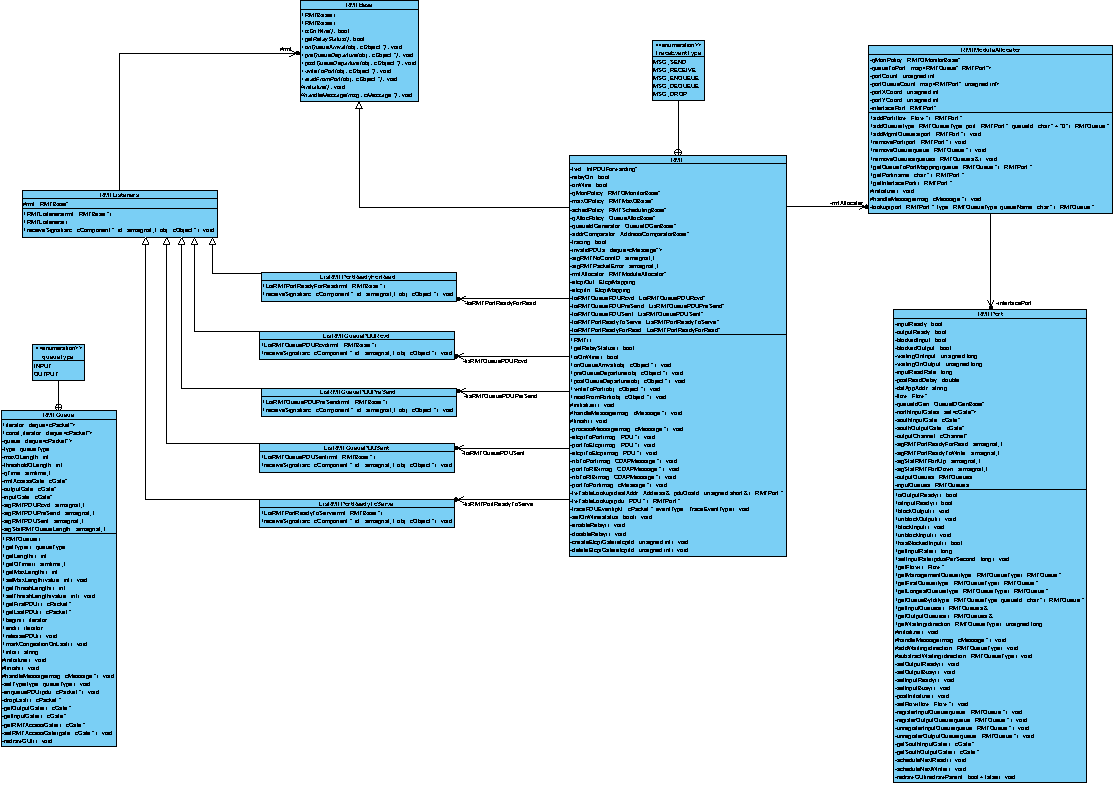
\includegraphics[angle=90,width=\textwidth]{fig/impl_rmt-erd.pdf}}
          \caption{RMT class diagram.}
          \label{fig:rinasim:rmt-erd}
        \end{center}
    \end{figure}